%========================================================
% EXPERIMENT 3 — Two-Arm PMD and Spectral-Correlation
%                Operating Regions
%========================================================

\subsection{Objective and Numerical Setup}

The third numerical experiment extends the single-arm analysis of
Section~\ref{sec:single_arm_pmd_operating_region} to the complete two-arm
configuration. The objective is to determine how PMD accumulated by both photons
combines with the spectral correlations of the entangled-photon source in
determining the BBM92 operating region.

The frequency offsets of photons \(A\) and \(B\) from their respective carrier
frequencies are denoted by

\begin{equation}
\Omega_A
=
\omega_A-\omega_{0,A},
\qquad
\Omega_B
=
\omega_B-\omega_{0,B}.
\label{eq:exp3_frequency_offsets}
\end{equation}

The joint spectral statistics of the two photons are described by a Gaussian
joint spectral intensity of the form

\begin{equation}
J(\Omega_A,\Omega_B)
\propto
\exp
\left[
-
\frac{(\Omega_A+\Omega_B)^2}
     {2\sigma_{\Sigma}^{\,2}}
-
\frac{(\Omega_A-\Omega_B)^2}
     {2\sigma_{\Delta}^{\,2}}
\right],
\label{eq:exp3_gaussian_jsi}
\end{equation}

where \(\sigma_{\Sigma}\) and \(\sigma_{\Delta}\) control the widths along the
sum- and difference-frequency directions, respectively.

For equal marginal spectral bandwidths,

\begin{equation}
\sigma_{\omega,A}
=
\sigma_{\omega,B}
=
\sigma_\omega,
\end{equation}

the spectral correlation coefficient is defined as

\begin{equation}
\boxed{
r
=
\frac{
\operatorname{Cov}(\Omega_A,\Omega_B)
}{
\sigma_\omega^2
},
\qquad
-1<r<1.
}
\label{eq:exp3_spectral_correlation_coefficient}
\end{equation}

With the Gaussian convention adopted in the simulator, the corresponding
sum- and difference-frequency widths are

\begin{equation}
\sigma_{\Sigma}
=
\sigma_\omega
\sqrt{2(1+r)},
\qquad
\sigma_{\Delta}
=
\sigma_\omega
\sqrt{2(1-r)}.
\label{eq:exp3_joint_spectral_widths}
\end{equation}

The parameter \(r\) therefore describes how the frequency offsets of the two
photons are statistically related. For \(r<0\), the frequencies are
anticorrelated: a positive frequency offset of one photon tends to be accompanied
by a negative offset of the other. For \(r>0\), the two offsets tend to have the
same sign and are positively correlated. The case \(r=0\) corresponds to
statistically uncorrelated frequency offsets.

Equivalently, negative \(r\) narrows the distribution along the
sum-frequency coordinate \(\Omega_A+\Omega_B\), whereas positive \(r\) narrows
it along the difference-frequency coordinate \(\Omega_A-\Omega_B\). The joint
spectral distribution therefore determines which combinations of photon
frequencies contribute most strongly to the propagated two-photon state.


%--------------------------------------------------------
% Frequency-Resolved Two-Photon States
%--------------------------------------------------------

\subsection{Generation of the Frequency-Resolved Polarization States}

The input polarization state is the Bell state

\begin{equation}
|\Psi^{+}\rangle
=
\frac{1}{\sqrt{2}}
\left(
|01\rangle+|10\rangle
\right),
\nonumber
\end{equation}

with density operator

\begin{equation}
\rho_{\mathrm{in}}
=
\ket{\Psi^+}
\bra{\Psi^+}.
\nonumber
\end{equation}

For every spectral pair
\((\Omega_A,\Omega_B)\), the polarization state is propagated through the two
frequency-dependent fiber transformations according to

\begin{equation}
\rho_{AB}(\Omega_A,\Omega_B)
=
U_{AB}(\Omega_A,\Omega_B)
\rho_{\mathrm{in}}
U_{AB}^{\dagger}(\Omega_A,\Omega_B),
\label{eq:exp3_frequency_resolved_state}
\end{equation}

where

\begin{equation}
U_{AB}(\Omega_A,\Omega_B)
=
U_A(\Omega_A)
\otimes
U_B(\Omega_B).
\label{eq:exp3_two_arm_unitary}
\end{equation}

Each arm is represented by one first-order PMD segment. Using the fiber model
introduced in Chapter~\ref{ch:02_fiber_channel_modeling}, the corresponding
unitary is

\begin{equation}
U_K(\Omega_K)
=
\exp
\left[
\frac{i}{2}
\Delta\tau_K
\Omega_K
\left(
\mathbf{n}_K\cdot\boldsymbol{\sigma}
\right)
\right],
\qquad
K\in\{A,B\},
\label{eq:exp3_single_arm_pmd_unitary}
\end{equation}

where \(\Delta\tau_K\) is the differential group delay and
\(\mathbf{n}_K\) is the local birefringence axis. The carrier-frequency
differential phase is set to zero in the present experiment so that only the
frequency-dependent PMD contribution is retained.

Both PMD axes are fixed along the same direction,

\begin{equation}
\mathbf{n}_A
=
\mathbf{n}_B
=
\hat{\mathbf{x}},
\label{eq:exp3_aligned_pmd_axes}
\end{equation}

so that the experiment isolates the effects of
\(\Delta\tau_A\), \(\Delta\tau_B\), and the spectral correlation \(r\).
Relative PMD-axis misalignment is investigated separately in the following
experiment.

The joint spectral distribution in
Eq.~\eqref{eq:exp3_gaussian_jsi} generates a statistical ensemble of
frequency-resolved polarization states. Since the photon frequencies are not
resolved in the polarization measurement, the reduced polarization density
operator is obtained by tracing over the spectral degree of freedom,

\begin{equation}
\boxed{
\rho_{\mathrm{pol}}
=
\iint
d\Omega_A\,d\Omega_B\,
P(\Omega_A,\Omega_B)
\rho_{AB}(\Omega_A,\Omega_B),
}
\label{eq:exp3_spectral_average}
\end{equation}

where

\begin{equation}
P(\Omega_A,\Omega_B)
=
\frac{
J(\Omega_A,\Omega_B)
}{
\displaystyle
\iint
d\Omega_A\,d\Omega_B\,
J(\Omega_A,\Omega_B)
}
\label{eq:exp3_normalized_jsi}
\end{equation}

is the normalized joint spectral probability distribution.

Numerically, the integral in Eq.~\eqref{eq:exp3_spectral_average} is evaluated
over the discrete spectral grid as

\begin{equation}
\rho_{\mathrm{pol}}
\simeq
\sum_{k,l}
Q_{kl}
\rho_{AB}
\left(
\Omega_{A,k},
\Omega_{B,l}
\right),
\label{eq:exp3_discrete_spectral_trace}
\end{equation}

where \(Q_{kl}\) are the normalized quadrature-weighted probabilities generated
from the Gaussian joint spectral intensity.

This construction makes the physical role of the source spectrum explicit.
Different values of \(r\) generate different statistical combinations of
\((\Omega_A,\Omega_B)\), which are subsequently converted by the two fiber
transformations into different distributions of polarization transformations.
The reduced polarization state therefore depends jointly on the source spectrum
and on the PMD parameters of both fiber arms.


%--------------------------------------------------------
% Physical Role of Spectral Correlation
%--------------------------------------------------------

\subsection{Physical Role of Spectral Correlation}

For the first-order model of Eq.~\eqref{eq:exp3_single_arm_pmd_unitary}, the
frequency-dependent differential phases accumulated in the two arms scale as

\begin{equation}
\delta\phi_A
=
\Delta\tau_A\Omega_A,
\qquad
\delta\phi_B
=
\Delta\tau_B\Omega_B.
\label{eq:exp3_two_arm_pmd_phases}
\end{equation}

Consequently, correlations between \(\Omega_A\) and \(\Omega_B\) translate
directly into correlations between the PMD-induced phase contributions.

For \(r<0\), the two frequency offsets preferentially have opposite signs.
When the two DGDs are comparable and the PMD axes are aligned, the corresponding
frequency-dependent contributions can therefore partially compensate. For
\(r>0\), the frequency offsets preferentially vary in the same direction and the
two PMD contributions instead tend to reinforce each other.

The two-arm PMD degradation is consequently determined not only by the
individual values of \(\Delta\tau_A\) and \(\Delta\tau_B\), but also by the
joint spectral structure of the photon pair. This is the principal physical
difference with respect to the single-arm configuration investigated in the
previous experiment.


%--------------------------------------------------------
% Numerical Parameter Space
%--------------------------------------------------------

\subsection{Numerical Parameter Space}

The marginal spectral bandwidth is fixed to

\begin{equation}
\sigma_\omega
=
1.0\times10^{11}
\;\mathrm{rad/s}.
\label{eq:exp3_sigma_omega}
\end{equation}

The two differential group delays are independently varied over

\begin{equation}
0
\leq
\Delta\tau_A,\Delta\tau_B
\leq
20
\;\mathrm{ps},
\end{equation}

using \(31\) points per arm.

Three representative spectral-correlation conditions are initially considered,

\begin{equation}
r=-0.9,
\qquad
r=0,
\qquad
r=+0.9,
\label{eq:exp3_representative_correlations}
\end{equation}

corresponding respectively to strongly anticorrelated, uncorrelated, and
strongly positively correlated spectra.

The spectral trace is evaluated using \(41\) frequency nodes per arm over the
interval

\begin{equation}
-6\sigma_\omega
\leq
\Omega_K
\leq
6\sigma_\omega.
\end{equation}

A second numerical sweep varies the spectral correlation continuously over

\begin{equation}
-0.9
\leq
r
\leq
0.9
\end{equation}

using \(37\) points, while restricting the fiber parameters to the symmetric
configuration

\begin{equation}
\Delta\tau_A
=
\Delta\tau_B
=
\Delta\tau.
\label{eq:exp3_symmetric_dgd_condition}
\end{equation}

For each resulting reduced polarization state, the basis-dependent BBM92 error
rates are evaluated and the operational metric is defined as

\begin{equation}
Q_{\mathrm{worst}}
=
\max
\left(
Q_Z,Q_X
\right).
\label{eq:exp3_worst_qber}
\end{equation}

The adopted operating condition is

\begin{equation}
\boxed{
Q_{\mathrm{worst}}
<
0.11.
}
\label{eq:exp3_bbm92_condition}
\end{equation}


%--------------------------------------------------------
% Two-Arm Operating Regions
%--------------------------------------------------------

\subsection{Two-Arm Operating Regions}

Figure~\ref{fig:exp3_two_arm_operating_regions} shows the resulting worst-basis
QBER in the \((\Delta\tau_A,\Delta\tau_B)\) plane for the three representative
spectral-correlation conditions.

\begin{figure}[htbp]
    \centering

    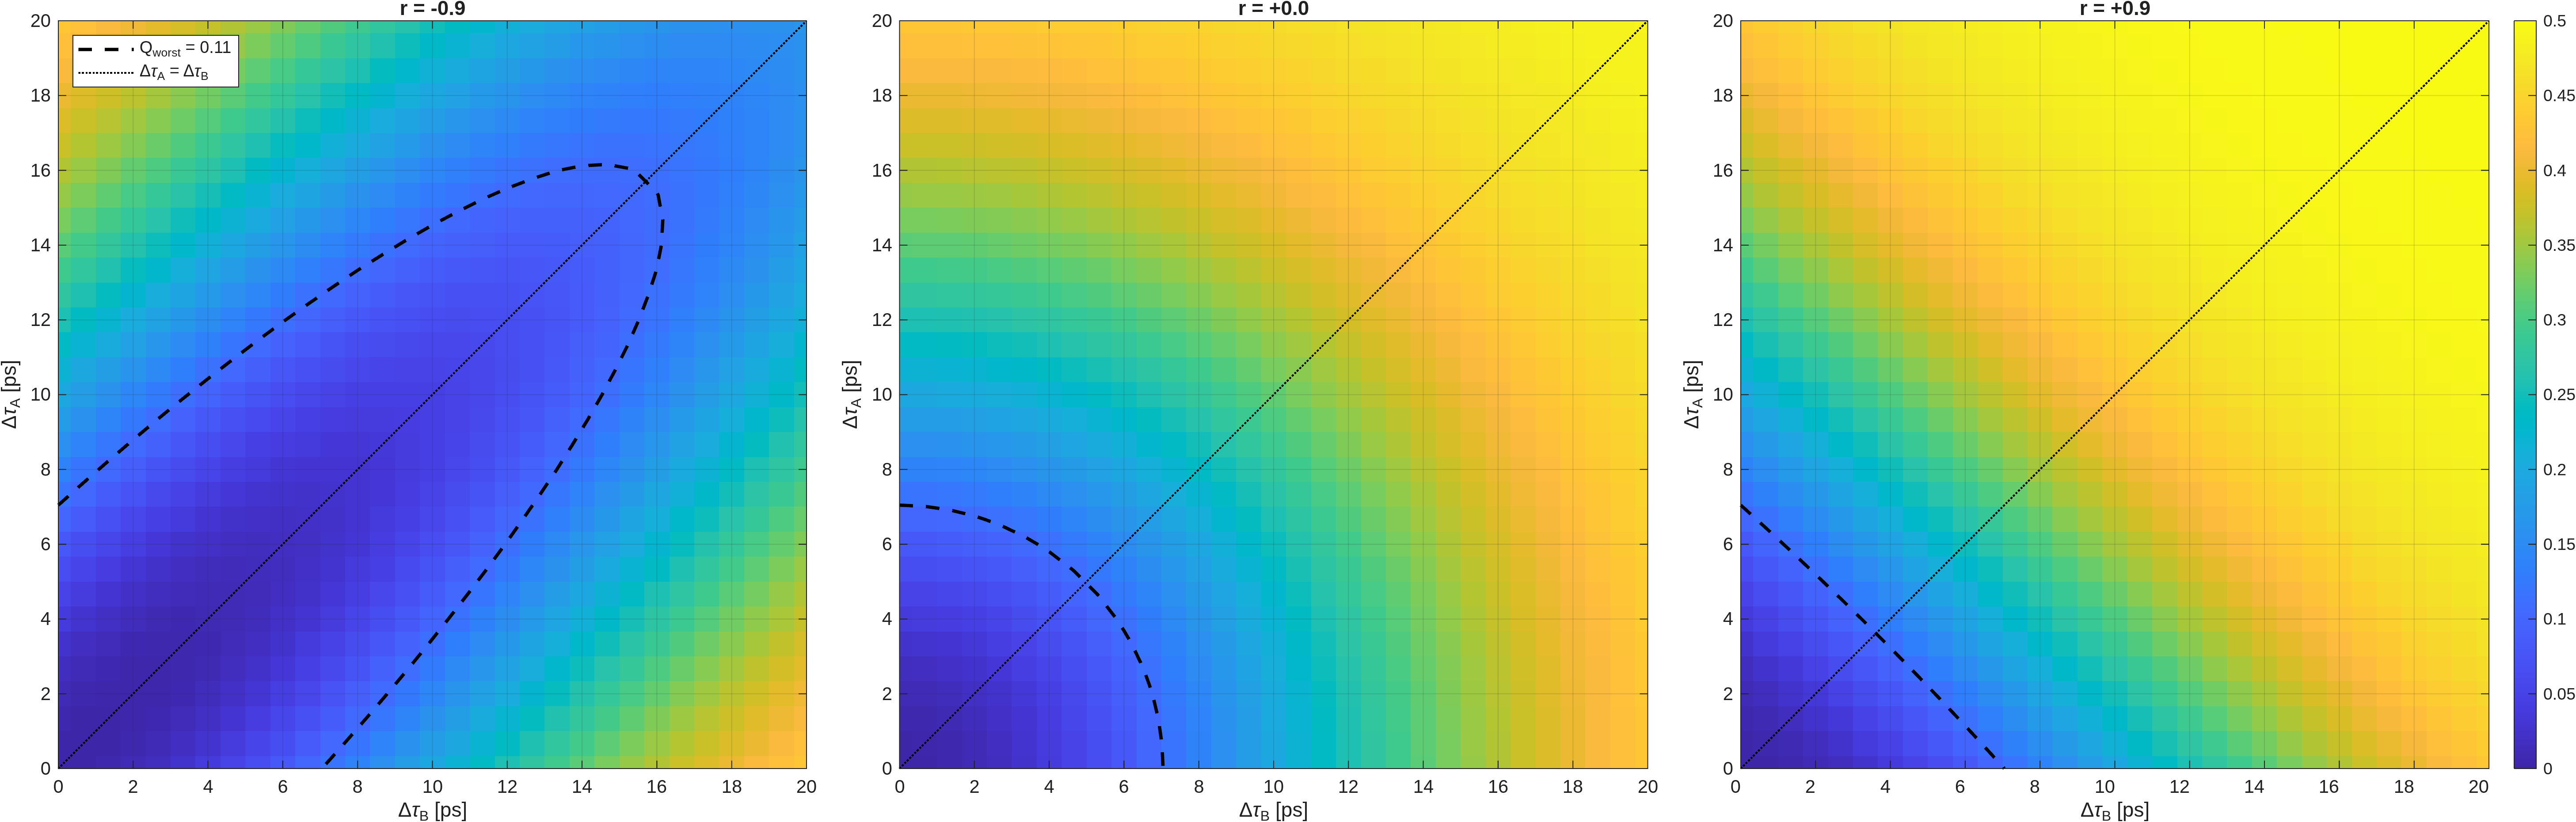
\includegraphics[
        width=\textwidth
    ]{
        figures/experiment_3/two_arm_pmd_operating_regions.png
    }

    \caption{
        Worst-basis BBM92 QBER as a function of the differential group delays
        \(\Delta\tau_A\) and \(\Delta\tau_B\) for strongly anticorrelated
        (\(r=-0.9\)), uncorrelated (\(r=0\)), and strongly positively
        correlated (\(r=+0.9\)) photon spectra. The dashed contour identifies
        the adopted operating boundary \(Q_{\mathrm{worst}}=0.11\), while the
        dotted line denotes the symmetric condition
        \(\Delta\tau_A=\Delta\tau_B\).
    }

    \label{fig:exp3_two_arm_operating_regions}
\end{figure}

The three panels show that spectral correlation changes not only the magnitude
of PMD-induced degradation but also the geometry of the two-arm operating
region.

For \(r=0\), the frequency offsets of the two photons are statistically
uncorrelated. Increasing the DGD in either arm therefore progressively increases
the effective polarization degradation, and the BBM92 operating region remains
concentrated around configurations in which the two DGDs are sufficiently
small.

For \(r=+0.9\), the two frequency offsets tend to have the same sign. For the
aligned PMD configuration considered here, the corresponding
frequency-dependent contributions tend to reinforce each other. The operating
region is consequently reduced when both arms simultaneously exhibit
significant DGD.

A qualitatively different behavior is observed for \(r=-0.9\). The frequency
offsets now preferentially have opposite signs. When the DGDs are comparable,
the two PMD-induced contributions can partially compensate. The BBM92 operating
region therefore extends toward substantially larger DGDs in the vicinity of

\begin{equation}
\Delta\tau_A
\simeq
\Delta\tau_B.
\end{equation}

The diagonal extension visible in the left panel is therefore a direct
consequence of the interaction between the anticorrelated source spectrum and
the frequency-dependent transformations of the two fiber arms. In particular,
large individual DGDs do not necessarily imply a correspondingly large
polarization degradation when their effects are correlated through the joint
spectrum.


%--------------------------------------------------------
% Symmetric-DGD Operating Boundary
%--------------------------------------------------------

\subsection{Spectral Correlation and Symmetric-DGD Tolerance}

The influence of spectral correlation is quantified more directly by restricting
the two-arm parameter space to

\begin{equation}
\Delta\tau_A
=
\Delta\tau_B
=
\Delta\tau
\end{equation}

and determining, for every value of \(r\), the maximum DGD compatible with the
adopted BBM92 criterion.

The resulting threshold
\(\Delta\tau_{\mathrm{th}}\) is shown in
Fig.~\ref{fig:exp3_spectral_correlation_boundary}.

\begin{figure}[htbp]
    \centering

    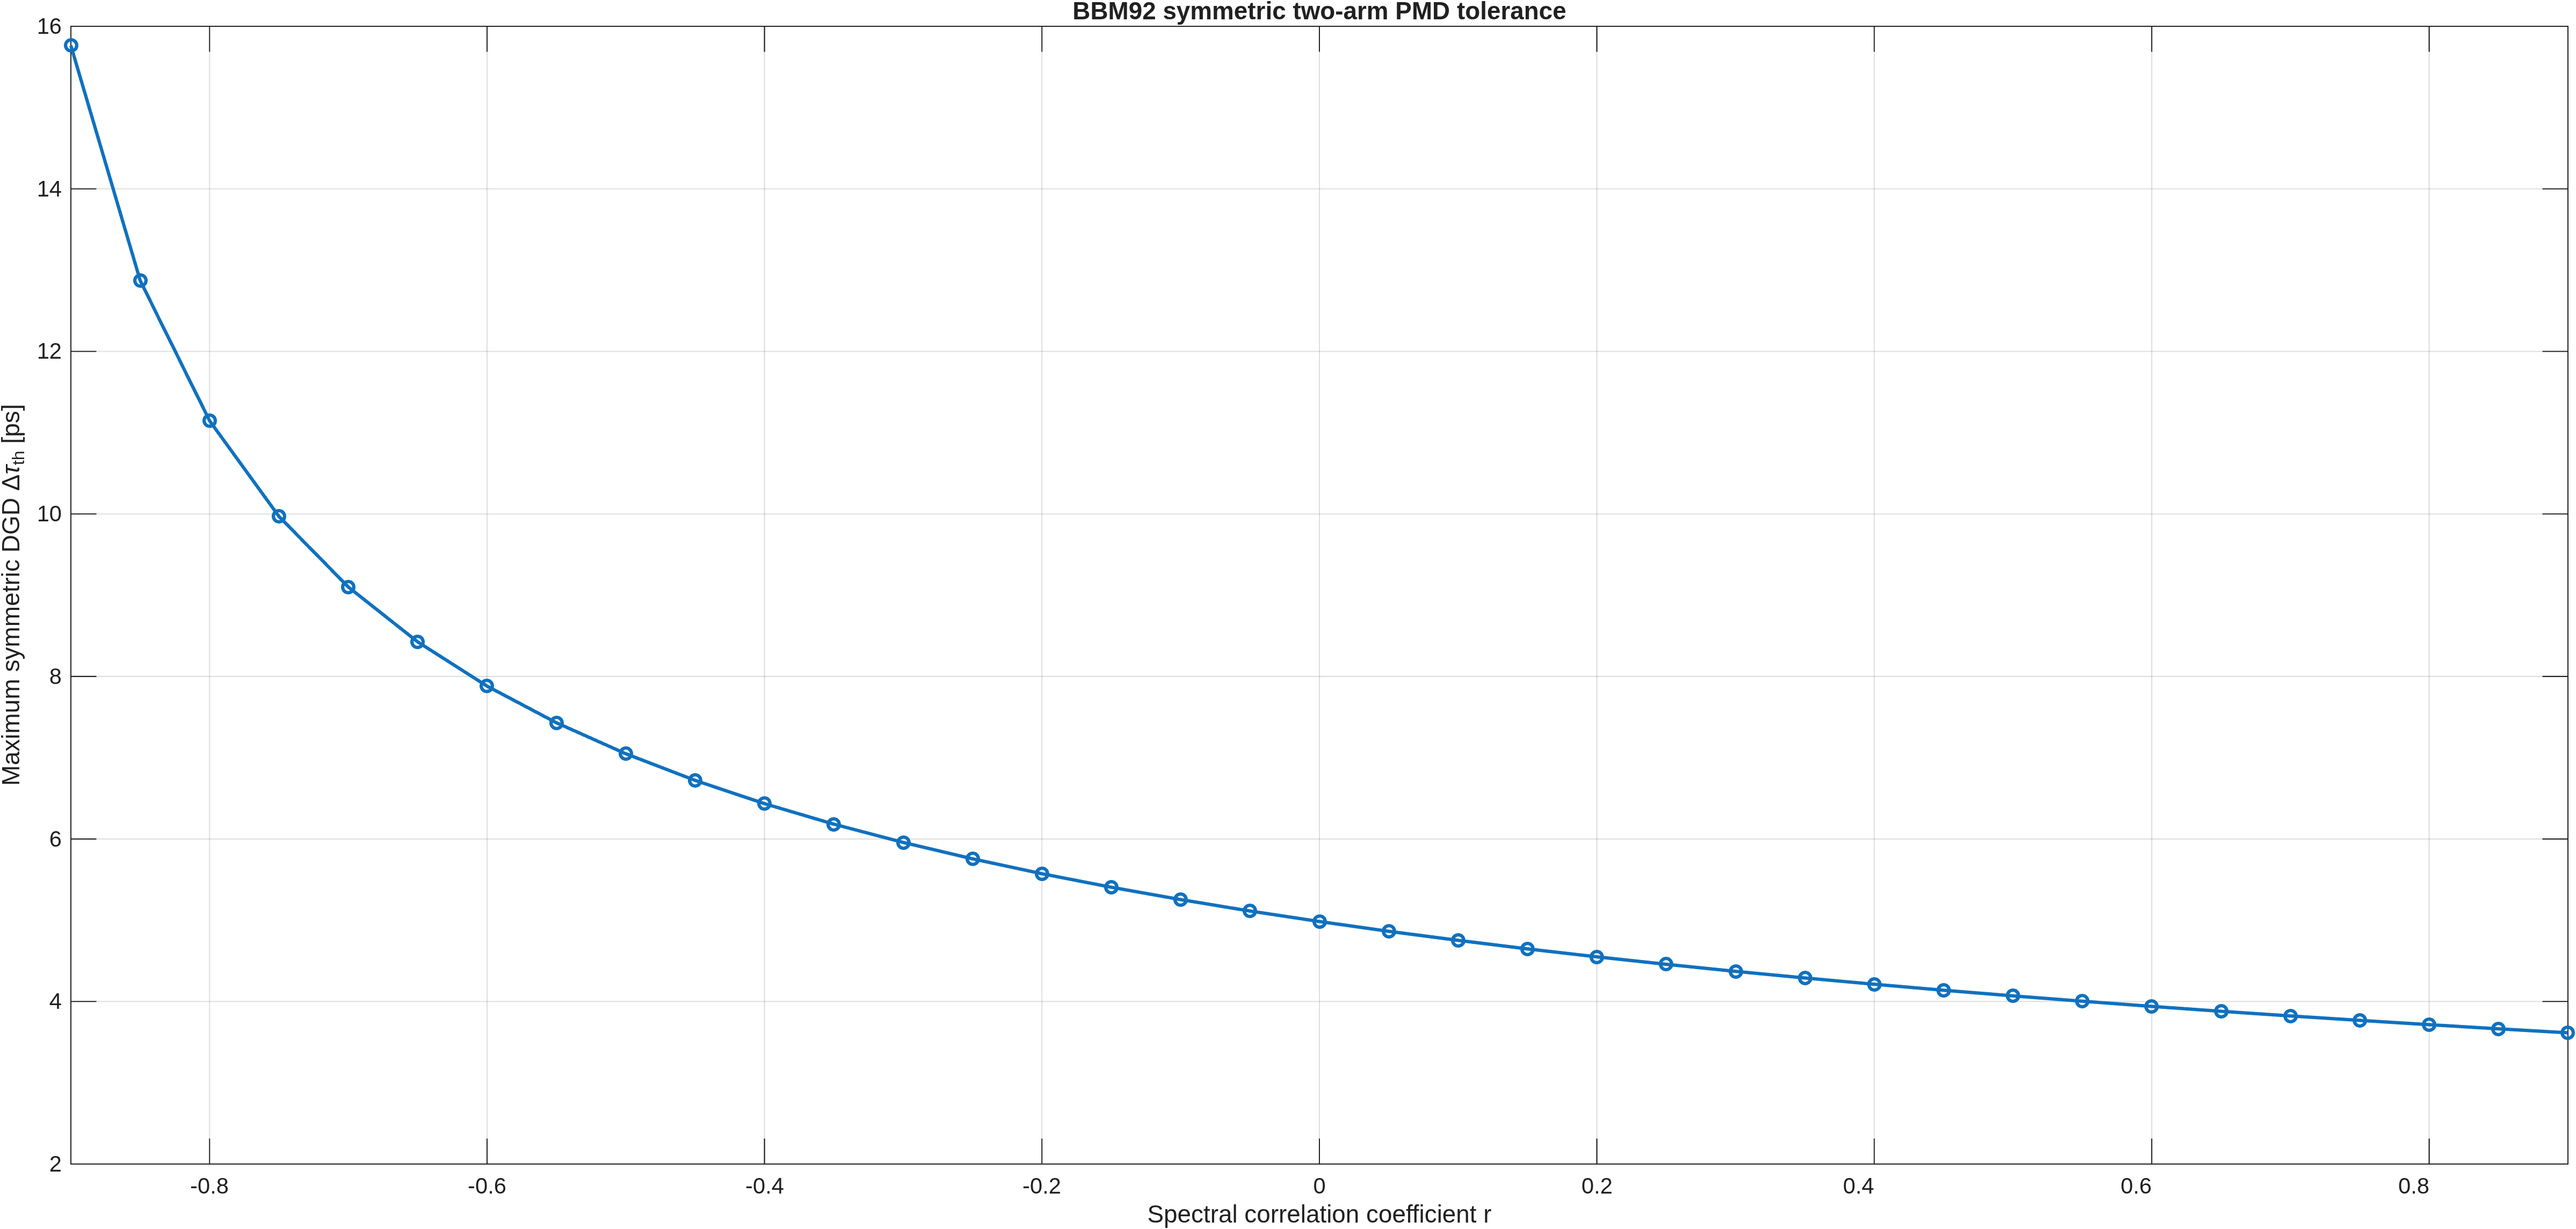
\includegraphics[
        width=0.88\textwidth
    ]{
        figures/experiment_3/spectral_correlation_dgd_boundary.png
    }

    \caption{
        Maximum symmetric differential group delay compatible with the adopted
        BBM92 operating condition as a function of the spectral correlation
        coefficient \(r\), for
        \(\sigma_\omega=1.0\times10^{11}\,\mathrm{rad/s}\).
        Negative spectral correlation substantially increases the tolerable
        symmetric DGD because the anticorrelated frequency offsets partially
        compensate the PMD contributions accumulated in the two aligned fiber
        arms.
    }

    \label{fig:exp3_spectral_correlation_boundary}
\end{figure}

The numerical boundary varies monotonically with the spectral correlation
coefficient. For the three representative conditions, the extracted threshold
DGDs are

\begin{equation}
\begin{aligned}
r=-0.9:
\qquad
\Delta\tau_{\mathrm{th}}
&=
15.763~\mathrm{ps},
\\
r=0:
\qquad
\Delta\tau_{\mathrm{th}}
&=
4.984~\mathrm{ps},
\\
r=+0.9:
\qquad
\Delta\tau_{\mathrm{th}}
&=
3.615~\mathrm{ps}.
\end{aligned}
\label{eq:exp3_symmetric_dgd_results}
\end{equation}

For the fixed source bandwidth considered here, the corresponding normalized
parameters

\begin{equation}
\chi_{\mathrm{th}}
=
\sigma_\omega
\Delta\tau_{\mathrm{th}}
\end{equation}

are

\begin{equation}
\chi_{\mathrm{th}}
=
1.5763,
\qquad
0.4984,
\qquad
0.3615,
\end{equation}

for \(r=-0.9\), \(r=0\), and \(r=+0.9\), respectively.

Moving from strong positive spectral correlation to strong spectral
anticorrelation therefore increases the maximum tolerable symmetric DGD from

\begin{equation}
3.615~\mathrm{ps}
\quad\text{to}\quad
15.763~\mathrm{ps},
\end{equation}

corresponding to an increase by more than a factor of four.

This improvement is obtained without changing either the marginal source
bandwidth or the individual PMD model of the two fibers. It originates entirely
from the different joint spectral statistics of the two photons and their
interaction with the frequency-dependent transformations accumulated in the two
arms.


%--------------------------------------------------------
% Operational Interpretation
%--------------------------------------------------------

\subsection{Operational Interpretation}

The concurrence evaluated at the numerically extracted BBM92 boundary is

\begin{equation}
C_{\mathrm{th}}
\simeq
0.7800
\end{equation}

for all three representative spectral-correlation conditions.

This value is not imposed as an entanglement threshold. The operating boundary
is determined exclusively from

\begin{equation}
Q_{\mathrm{worst}}
=
0.11,
\end{equation}

and the concurrence is evaluated only after the corresponding physical
configuration has been identified. The approximately constant value
\(C\simeq0.78\) is therefore a property of the restricted aligned-axis Gaussian
state family considered here and must not be interpreted as a universal
concurrence requirement for BBM92 operation.

The main result of the experiment is instead that two-arm PMD cannot generally
be characterized by the individual DGDs alone. The same pair of fiber
parameters can produce substantially different polarization degradation
depending on the spectral correlation of the entangled-photon source.

The physical-to-operational mapping investigated in this experiment can
therefore be summarized as

\begin{equation}
\boxed{
\left(
\Delta\tau_A,
\Delta\tau_B,
r
\right)
\longrightarrow
\rho_{\mathrm{pol}}
\longrightarrow
Q_{\mathrm{worst}}
\longrightarrow
\mathcal{R}_{\mathrm{BBM92}}.
}
\label{eq:exp3_final_parameter_mapping}
\end{equation}

Spectral correlation thus becomes an additional source parameter controlling the
robustness of the distributed polarization state against two-arm PMD. In the
specific aligned configuration considered here, strong spectral anticorrelation
can substantially enlarge the BBM92 operating region when the differential group
delays of the two arms are appropriately matched.